\documentclass[svgnames,a4paper,11pt,fleqn,openright]{report}
\usepackage[table]{xcolor}
\usepackage{xparse,tikz}
\usepackage{pgffor}
\usetikzlibrary{positioning}
\usepackage{verbatim}
\usepackage{nameref}
\usepackage{parskip}
\definecolor{light-gray}{gray}{0.8}
\usepackage{array}
\usepackage[compact, explicit]{titlesec}
\usepackage{pdfpages}
\usepackage{colortbl}
\usepackage{url}
\usepackage[utf8]{inputenc}
\usepackage{listingsutf8}
\usepackage{listings}
\usepackage{amsfonts}
\usepackage{amsmath}
\usepackage{amssymb}
\usepackage{longtable} 
\usepackage{pdflscape}
\usepackage{makecell}
\usepackage[]{todonotes}
\marginparwidth = 105pt
\usepackage{wrapfig}
\usepackage{blindtext}
\usepackage{tabularx}
\usepackage{float}
\usepackage{changepage}
\usepackage{pbox}
\usepackage{rotating}
\usepackage{textcomp}
\usepackage{fourier}
\usepackage{color}

\usepackage[backend=bibtex,sorting=none]{biblatex}
\addbibresource{misc/litteratur.bib}

\newcommand*\chapterlabel{}
\titleformat{\chapter}
  {\gdef\chapterlabel{}
   \normalfont\sffamily\Huge\bfseries\scshape}
  {\gdef\chapterlabel{\thechapter.\ }}{0pt}
  {\begin{tikzpicture}[remember picture,overlay]
    \node[yshift=-2cm] at (current page.north west)
      {\begin{tikzpicture}[remember picture, overlay]
        \draw[fill=light-gray] (0,0) rectangle
          (\paperwidth,2cm);
        \node[anchor=east,xshift=.9\paperwidth,rectangle,
              rounded corners=20pt,inner sep=11pt,
              fill=Gray]
              {\color{white}\chapterlabel#1};
       \end{tikzpicture}
      };
   \end{tikzpicture}
  }
\titlespacing*{\chapter}{0pt}{10pt}{-80pt}
\titlespacing*{\section}{0px}{20pt}{-10px}
\titlespacing*{\subsection}{0px}{20pt}{0px}
\titleformat{\section}{\Large\bfseries}{\thesection}{1em}{#1\hrule}

% ¤¤ Visuelle referencer ¤¤ %
\usepackage[colorlinks]{hyperref}			 	% Giver mulighed for at ens referencer bliver til klikbare hyperlinks. .. [colorlinks]{..}
\hypersetup{pdfborder = 0}							% Fjerner ramme omkring links i fx indholsfotegnelsen og ved kildehenvisninger ¤¤
\hypersetup{														%	Opsætning af hyperlinks
    colorlinks = false,
    linkcolor = black,
    anchorcolor = black,
    citecolor = black
}

\setcounter{tocdepth}{1}
\makeatletter
\renewcommand{\l@section}{\@dottedtocline{1}{1.5em}{3.0em}}
\makeatother

\definecolor{commentColor}{rgb}{0,0.4,0}
\definecolor{keywordColor}{rgb}{0,0,1}
\definecolor{stringColor}{rgb}{0.5,0,0.5}
\definecolor{numberColor}{rgb}{0.2,0.2,0.2}

\lstset{
  language=c++,
  frame=single,
  keywordstyle=\color{keywordColor},
  commentstyle=\color{commentColor},
  stringstyle=\color{stringColor},
  numberstyle=\color{numberColor},
  captionpos=b,
  numbers=left,
  numbersep=8pt,
  tabsize=2
}

% include this to show boxes
%\usepackage{showframe}
\begin{document}


\includepdf{misc/title.pdf}
\thispagestyle{empty}

{\samepage 
\begin{tabular}{r}
	\parbox{\textwidth}{ {
\includegraphics[scale=0.5]{misc/aauLogoEn.png}}
	\hfill \parbox{7cm}{\begin{tabular}{l} %4.90
		{\small \textbf{Department of Computer Science}}\\
		{\small Selma Lagerlöfs Vej 300} \\
		{\small 9220 Aalborg Ø}
	\end{tabular}}
	}
\end{tabular}

\begin{tabular}{cc}
	\parbox{7cm}{
	\begin{description}
		\item { \textbf{Title:}}\\ 
			YAGAL: Yet Another GPGPU Abstraction Library
    		\item { \textbf{Theme:}}\\ 
			Programming Technology\\
	\end{description}
	
	\parbox{7cm}{
	\begin{description}
		\item { \textbf{Project period:}}\\
			01/02/2018 -\\
			08/06/2018\\
 		\hspace{4cm}
		\item { \textbf{Project group:}}\\
  			DPW10618\\
 		\hspace{4cm}
		\item {\textbf{Members:}}\\
            Jonathan Hastrup\\
            Morten Mandrup Hansen\\
		\hspace{2cm}
		\item { \textbf{Supervisor:}}\\
 			Lone Leth Thomsen\\
  	\end{description}
	}

	\begin{description}
		\item { \textbf{No. of Pages: } ?? } 
		\item { \textbf{No. of Appendix Pages: } ?? }
		\item { \textbf{Total no. of pages: } ??+?? } 
		\item { \textbf{Completed:} 08/06/2018}
	\end{description}
	\vfill } &
	\parbox{6.5cm}{
 	 \vspace{.15cm}
  	\hfill 
  	\begin{tabular}{l}
  		%{ Abstract:}
		  \bigskip \\
  		\fbox{
  		\parbox{7cm}{\bigskip
     		{\vfill{\small General purpose GPU(GPGPU) programming require a developer to learn how to program in a new programming model to be effective. There are already related work addressing GPGPU, but they either utilize a custom compiler, and thereby enforcing the choice of compiler for the developer, or they utilize \textit{OpenCL} as a target language.
This report documents the development of \textit{YAGAL}, a GPGPU abstraction library, that utilize the \textit{CUDA Driver API} for device management, and \textit{LLVM} for \textit{PTX} code generation at run-time, to be compiler independent without relying on \textit{OpenCL}.
With the library, we explore the option of building kernels though an action abstraction that allow chaining of function invocations on a vector object to generate and execute a kernel on the GPU.
We compare the framework to the state of the art, in terms of both static measurements, and usability by using Cognitive Dimensions of Notations.
We reflect upon our thesis work in terms of technology choice, selected related works, framework implementation and comparison process.
We conclude that development of a GPGPU framework is indeed possible with the configuration used, but that it might not be worth the development effort involved, when other options appear as equally good options with simpler development.
     		\bigskip}}
     	}}
   	\end{tabular}}
\end{tabular}
}

\chapter*{Preface}
\section*{Reading Instructions}
\todo{write this}

Left to right, top down. Pretty straight forward.

\section*{Definitions}
This is a list of terms heavily used in this report, with their definitions.

\begin{description}
\item[GPU] Graphics Processing Unit.
\item[GPGPU development] General Purpose GPU development. To develop general purpose applications targetting GPU hardware.
\item[STL] The C++ Standard Template Library.
\end{description}


\tableofcontents

\chapter{Introduction}
%what are we doing
We propose an abstraction library that allows a developer to quickly explore the potential of a GPU enhanced program.
\section{Motivation}
In our SW9 project we experienced that it is difficult to get started with OpenCL/CUDA development. There are multiple new concepts to learn, such as the programming model with kernels, and the memory model of the GPU. This means that a developer who believe, that the performance of an application can be improved by utilizing a GPU, need to learn all of this before being able to test his theory. This is difficult and we want to be able to initially abstract away all most of the GPU computing model until the developer is ready to learn it.

\todo[inline]{find andre der har svært ved dette, eller nogen der kan bakke vores problem påstand op.}
\section{Problem Statement}
What we exactly want to solve

What we do not attempt to achieve:
Outperform openCL and CUDA performance wise. 
\section{Development Process}
In section \ref{cha:tasks}, we define the tasks that need to be done to reach the goals in our problem statement. These tasks have a linear dependency which motivates us to follow a waterfall inspired development process. This process is separated into two major parts; Design and implementation of our framework, and comparison between our framework and other frameworks. 

During design and implementation, some features might be iterated multiple times, but when this happens it will be made clear. Before we start the comparison part, we will have completed the design and implementation part.

%The parts each cover multiple sub parts, chosen to perform the tasks mentioned in Chapter \ref{cha:tasks}. The report follows the structure of these parts to document the process.\todo{gør dette sandt.} The parts and sub parts consist of:
%\begin{description}
%\item[Design and implementation of our framework] \hfill
%\begin{itemize} 
%\item Research of related works.
%\item Designing our framework.
%\item Implementation of our framework.
%\item Test of our framework.
%\end{itemize}
%\item[Comparison between our framework and other frameworks] \hfill
%\begin{itemize} 
%\item Research of comparison methodology.
%\item Implementation of demo application in our framework.
%\item Implementation of the same demo applications in other frameworks.
%\item Comparing implementations.
%\item Comparing the frameworks.
%\item Evaluation of our framework.
%\end{itemize}
%\end{description}


\chapter{Related Works}
Before we design our framework, we consider other frameworks that attempt to reach similar goals. This allow us to make more informed decisions when we design our framework, as we then know how others have approached similar problems, and what their result was. We also learn how others have provided abstractions for the underlying architecture, giving us inspiration for our API design.

%We consider related work to be able to have a better understanding of different problems and solutions that other have encountered while creating GPGPU frameworks. We will select relevant frameworks, and interesting topics where others previous experience can help us.

\section{Selection of Related Works}
In our previous project, we compared multiple languages supporting development targeting the GPU\cite{sw9Report}. We observed how \textit{CUDA} and \textit{OpenCL} was the frameworks that offered the most explicit device control, and as such can be the choice for people with knowledge of how to fine tune a GPGPU application. As we intend to make a framework that should be able to be replaced by a low level programming model, and \textit{CUDA} or \textit{OpenCL} seem to be the dominant options, we want to get an overview of other frameworks targeting the host language of \textit{CUDA} and \textit{OpenCL}, being \textit{C} and \textit{C++}.

The frameworks we examine are:
\begin{description}
\item[Thrust] \hfill \\
Being promoted by \textit{NVIDIA}, developer of \textit{CUDA}, as a high level interface to GPU Programming, it is interesting to us\cite{thrustNvidia}.
\item[C++ Amp] \hfill \\
Being promoted by \textit{Microsoft}, developer of \textit{DirectX}, as a \textit{C++} language extension to enable data-parallel acceleration, it is interesting to us\cite{microsoftCppAMP}.
\item[SYCL] \hfill \\
Being promoted by \textit{Khronos Group}, developer of \textit{OpenCL}, as a abstraction layer that allow use of \textit{OpenCL} as a platform with standard \textit{C++} on both host and device\cite{khronosSYCL}.
\item[Bolt] \hfill \\
It is developed by the \textit{HSA Foundation} to provide a high level library to provide abstractions on top of low level programming models. As the goal is similar to ours it is interesting\cite{boltDoc}.
\item[SkelCL] \hfill \\
It is a research project that attempts to make GPU development easier with a concept called algorithmic skeletons. As the goal is similar to ours it is interesting\cite{skelclPaper}.
\item[PACXX] \hfill \\
It is a research project that attempts to make GPU development easier by combining host and device code in standard \textit{C++}. As the goal is similar to ours it is interesting\cite{pacxxPaper}.
\end{description}

The libraries are being considering in regards to:
\begin{description}
\item[Goals] \hfill \\
To identify the motivation for the framework and to understand the motivation behind its design choices.
\item[Programming Model] \hfill \\
To identify the programming model of a framework to see which aproaches have been tried, and what is currently possible. To give a demonstration of the programming model, an implementation of the \textit{SAXPY} computation is presented for each. We chose \textit{SAXPY} due to its simplicity.
\item[Implementation] \hfill \\
To identify the means of facilitating the programming model, showing how it can be done.
\item[Key Points] \hfill \\
To identify relevant points to note from a framework, that should be considered when designing our framework.
\end{description}
\section{Thrust}
\textit{Thrust} is a \textit{C++} library that allow developers to implement high performance applications with minimal programming effort. This section is based on \textit{Thrust}'s overview document\cite{thrustOverview} and \textit{Github} page\cite{thrustGithub}.

\subsection{Goals}
The aim of \textit{Thrust} is to make high performance application development as easy as possible. It is designed to be similar to \textit{STL}, with the intention of being concise, readable, and efficient. It is intended to supply the developers with containers and fundamental algorithms, with user defined behavior, rather than specific numeric algorithms as provided by \textit{BLAS}. It is also intended to be interoperable with \textit{CUDA}.

\subsection{Programming Model}
\textit{Thrust} is modeled on \textit{STL} and as such, follows the model of calling functions with iterators as arguments to instruct where input, and output is located.

Listing \ref{code:thrustSaxpy} shows how the \textit{SAXPY} computation can be implemented in \textit{Thrust}, and the usage of iterators to manage data access is shown.

The execution of \textit{SAXPY} is done in line \ref{code:thrustSaxpy:execute}, and shows how iterators are used to define input and output locations.
\begin{lstlisting}[caption={\textit{Thrust} \textit{SAXPY} example.}, label={code:thrustSaxpy}]
size_t N = 1024;
int a = 10;

//cuda classifier on lambda
auto func = [=]__device__(int x, int y){return a * x + y;};

//initialize host vectors
thrust::host_vector<int> x(N);
thrust::host_vector<int> y(N);
thrust::host_vector<int> z(N);

//fill with random data
std::generate(x.begin(), x.end(), rand);
std::generate(y.begin(), y.end(), rand);

//copy to device
thrust::device_vector<int> d_x = x;
thrust::device_vector<int> d_y = y;

//perform saxpy
thrust::transform(d_x.begin(), d_x.end(), d_y.begin(), d_y.begin(), func); ~\label{code:thrustSaxpy:execute}~

//copy results back to host vector
z = d_y;
\end{lstlisting}

\subsection{Implementation}
\textit{Thrust} is a library build on top of the \textit{CUDA} library. This means that the developer will include the \textit{Thrust} header files needed, and compile her program with the \textit{NVIDIA} compiler, \textit{nvcc}, as seen on \ref{fig:thrustCompilation}. 

The memory management is performed though types defined in the library, abstracting away direct allocation management, and functions can be defined as lambdas with the annotation \textit{\_\_device\_\_} which is the \textit{CUDA Runtime} annotation for kernels. With \textit{nvcc} as the compiler thrust can achieve the high level design shown in listing \ref{code:thrustSaxpy}, where the thrust data types interface with \textit{STL} algorithms and use close to pure \textit{C++11} syntax for lambdas.

The compilation process is static, and results in a single executable with both host and \textit{CUDA Runtime} code included.
\begin{figure}[H]
\center
\includegraphics[width=0.8\textwidth]{chapters/relatedWorks/figures/thrust_compilation.png}
\caption{Thrust Compilation Process.}
\label{fig:thrustCompilation}
\end{figure}

\subsection{Key Points}
The API of \textit{Thrust} is structured to imitate that of \textit{STL}, and a \textit{C++} developer is therefore familiar with it. It can be very verbose with multiple operations on the same container since the usage of the containers is based on iterators.

\textit{Thrust} is a header only implementation, meaning there is no need for a specialized compiler, and it builds upon \textit{CUDA}. This allows mixing \textit{Thrust} and \textit{CUDA} code if there is a need for specialized code.
\section{C++ AMP}
\textit{AMP} stands for Accelerated Massive Parallelism, and is a runtime library that allows a developer to write code to be executed on data-parallel hardware and is built upon \textit{DirectX 11}. \textit{C++ AMP} is developed by \textit{Microsoft} as a library and as an open standard for implementing parallelism in \textit{C++}. Their choice of \textit{DirectX 11} is interesting since \textit{OpenCl} and \textit{CUDA} existed at the time. The information discussed in this section was gained from \textit{Microsoft}'s \textit{C++ AMP} page \cite{microsoftCppAMP}.

% The commented text describes an implementation outputting OpenCL
% which have led to the announcement from the \textit{HSA Foundation} about an AMP compiler built with \textit{Clang}\cite{clang} and \textit{LLVM}\cite{llvm} that outputs to \textit{OpenCL} instead of DirectX11.

\subsection{Goals}
The aim of the \textit{C++ AMP} specification is to provide a way of writing code for data parallel hardware directly within the \textit{C++} language. \textit{Microsoft} implemented the specification based upon \textit{DirectX 11}, and the \textit{HSA Foundation} later did it for \textit{OpenCL}.

\subsection{Programming model}
A feature of \textit{C++ AMP} is that kernel functions is here expressed in \textit{C++} as restricted lambdas, meaning that a subset of \textit{C++} is available. 

Construction of matrices is done by first creating an array, and then wrap it with the \texttt{array\_view} that is provided by \textit{C++ AMP}. To show an example, an array is constructed below:
\begin{lstlisting}
int matrix[] = {1, 2, 3, 4}; 
\end{lstlisting}
To construct a matrix with two dimensions, the \texttt{matrix} array is wrapped with \texttt{array\_view}:
\begin{lstlisting}
array_view<int, 2> mat(2, 2, matrix); 
\end{lstlisting}
Here the \texttt{<int, 2>} specifies that the \texttt{mat} matrix consist of integers and two dimensions. \texttt{(2, 2, matrix)} indicates that the \texttt{mat} matrix will have two rows and two columns, and will be populated with the data from the \texttt{matrix} array;

Listing \ref{code:cppampSaxpy} shows \textit{SAXPY} implemented in \textit{C++ AMP}. The \texttt{array\_view}s are constructed at line \ref{code:cppampSaxpy:viewsStart} to \ref{code:cppampSaxpy:viewsEnd}. It is still needed to specify the views, even though this example only utilize one dimension. The \texttt{z\_v} \texttt{array\_view} is at line \ref{code:cppampSaxpy:discard} marked with the \texttt{discard\_data()} function. This is done to indicate that \texttt{z\_v} is used purely as an output container, and to avoid wasting resources transferring it to device since the contents will be overwritten.
At line \ref{code:cppampSaxpy:forEach} the function \texttt{parallel\_for\_each()} method is called and given two arguments. \texttt{z\_v.extend} indicates the compute domain. The lambda at line \ref{code:cppampSaxpy:lambda} are marked with \texttt{restrict(amp)} which states that the lambda should be executed on device and that only a subset \textit{C++} functionality is available for execution.
\begin{lstlisting}[caption={\textit{C++ AMP} \textit{SAXPY} example.}, label={code:cppampSaxpy}]
const size_t N = 1024;
int a = 10;

std::array<int, N> x;
std::array<int, N> y;
std::array<int, N> z;

std::generate(x.begin(), x.end(), rand);
std::generate(y.begin(), y.end(), rand);

array_view<const int, 1> x_v(size, x);~\label{code:cppampSaxpy:viewsStart}~
array_view<const int, 1> y_v(size, y);
array_view<int, 1> z_v(size, z);~\label{code:cppampSaxpy:viewsEnd}~
z_v.discard_data();~\label{code:cppampSaxpy:discard}~

parallel_for_each( ~\label{code:cppampSaxpy:forEach}~
    z_v.extent,

    [=](index<1> idx) restrict(amp){ ~\label{code:cppampSaxpy:lambda}~
        z_v[idx] = a * x_v[idx] + y_v[idx];
    }
)
\end{lstlisting}

\subsection{Implementation}

% Intro / Overview
\textit{C++ AMP} is a library that enables simple manipulation of large dimensional arrays by introducing a new language feature called \texttt{restricted} for \textit{C++}. 

% Memory / Types
Data are managed within regular \texttt{std::array}s. \texttt{array\_view}s are then constructed to represent these arrays as matrices on the GPU and used to manipulate them.

% Kernels / Fame?
Lambdas are used to construct the logic of a kernel for execution on the GPU. The \texttt{restricted} keyword are used in conjunction upon the lambda to indicate for the compiler that not all functionality are available within the scope of this lambda. 

To execute the kernel, the lambda are given to the \texttt{parallel\_for\_each} function that first copies the data described by the \texttt{array\_views} to the GPU and then executes the lambda.

% Comp / Figref
The compilation chain of \textit{C++} AMP can be seen in Figure \ref{fig:cppampCompilation}. Here the user code have included the \textit{C++ AMP} headers and compiled by the \textit{Microsoft Visual C++} compiler (\textit{MSVC}). The result is a executable file that utilizes \textit{Direct3D} to execute on the GPU. Even though \textit{C++ AMP} is an includeable library, it makes use of compiler specific functionality to add an additional keyword to the language and is therefore tied to the \textit{MSVC} compiler for \textit{windows}. The \textit{C++ AMP} specification is however open such that other compiler vendors could support it in the future.

\begin{figure}[H]
\center
\includegraphics[width=0.8\textwidth]{chapters/relatedWorks/figures/cppamp_compilation.png}
\caption{C++ AMP Compilation Process.}
\label{fig:cppampCompilation}
\end{figure}

\subsection{Key Points}
A unique feature of \textit{C++ AMP} is that it outputs to \textit{DirectX11}. We assume that this decision might have been made due to DirectX11 being developed and maintained by \textit{Microsoft} as well.

\textit{C++ AMP} is meant to extend \textit{C++} with parallelism. While this allows a developer to write code for GPUs in \textit{C++}, there are still some quirks in the form of \textit{array\_view} and restricted lambdas.

\section{SYCL}
\textit{SYCL} is a high-level programming language that provide an abstraction layer for \textit{OpenCL} and it is developed by \textit{Khronos Group}. This section describes \textit{SYCL} based on the information available at the \textit{Khronos Group} website \cite{khronosSYCL}.

\subsection{Goals}
As opposed to regular \textit{OpenCL} devlopment, \textit{SYCL} enables the host and device code to be contained within a single source. \textit{SYCL} exposes the \textit{OpenCL} feature-set with a higher abstraction level, as well as most modern \textit{C++} features. 

The \textit{Khronos Group} aim to follow the current \textit{C++} standard developments and integrate it with \textit{OpenCL} features.

\subsection{Programming model}
\textit{OpenCL} has commands for memory object creation, copying, mapping and synchronisation. \textit{SYCL} wraps these as a \textit{command group} that can manage these commands. Listing \ref{code:saxpySycl} shows a sample with an implementation of the \textit{SAXPY} computation. \textit{SYCL} need to know which variables should be available for device use, and this is indicated by firstly setting up host storage as seen through line one to three. These variables, \texttt{x}, \texttt{y}, and \texttt{z}, are then placed in a buffer, as seen on lines five to seven, which marks the data to be shared between host and device and initializes the queue. Next, at lines nine and ten, the available decises are registered by initializing the \texttt{device\_selector}. At line 12 the buffer elements are submited by the \texttt{cgh} handler, and at following three lines it is specified how each buffer element should be accessed; \texttt{x} and \texttt{y} is set with the \textit{read} access mode and \texttt{z} is set with the \textit{discard\_write} access mode. The actual execution of \textit{SAXPY} is specified at lines 17 and 18.

\begin{lstlisting}[caption={\textit{SAXPY} implemented in \textit{SYCL}.}, label={code:saxpySycl}]
sycl::float4 x = { 1.0, 2.0, 3.0, 4.0 };
sycl::float4 y = { 2.0, 3.0, 4.0, 5.0 };
sycl::float4 z = { 0.0, 0.0, 0.0, 0.0 };

sycl::buffer<sycl::float4, 1> a_sycl(&x, sycl::range<1>(1));
sycl::buffer<sycl::float4, 1> a_sycl(&y, sycl::range<1>(1));
sycl::buffer<sycl::float4, 1> a_sycl(&z, sycl::range<1>(1));

sycl::default_selector device_selector;
sycl::queue queue(device_selector);

queue.submit([&] (sycl::handler& cgh) {
  auto x_acc = x_sycl.get_access<sycl::access::mode::read>(cgh);
  auto y_acc = y_sycl.get_access<sycl::access::mode::read>(cgh);
  auto z_acc = z_sycl.get_access<sycl::access::mode::discard_write>(cgh);

  cgh.single_task<class saxpy>([=] () {
    z_acc[0] = 2 * x_acc[0] + y_acc[0];
  });
});
\end{lstlisting}

Even though \textit{SYCL} provides a higher abstraction level compared to regular \textit{OpenCL}, low-level \textit{C++} and \textit{OpenCL} features are still available.

\subsection{Implementation}
Primarily targets \textit{OpenCL}, but can also target other backends as it is translated to \textit{SPIR-V}, which an imediate representation.

\subsection{Key Points}
A key point of \textit{SYCL} to make note of is its way of specifying data that should be available for host and devices. By placing data in the buffers and specifying how the data should be accessed, shown in listing \ref{code:saxpySycl} as \texttt{read} and \texttt{discard\_write}, the availability of data is clear. 

Another point to note, that is different than the approaches of the other libraries, is that the parallel logic is structured similar to how a kernel function would be in \textit{OpenCL}/\textit{CUDA} instead of it being abstracted away.

\section{Bolt}
\textit{Bolt} is a library providing abstractions for heterogeneous computing. This section is based on \textit{Bolt}'s documentation\cite{boltDoc} and \textit{Github} page\cite{boltGithub}.

\subsection{Goals}
\textit{Bolt} is aim to provide high performance library implementations for common algorithms, following the structure of \textit{STL}. It is intended to make heterogeneous development easieran, and is designed to provide an application that can execute on either a CPU or any OpenCL capable unit.

\subsection{Programming Model}
\textit{Bolt} is modeled on \textit{STL} and as such, follows the model of calling functions with iterators as arguments to instruct where input and output is located.

It have functions for modifying \textit{STL} containers, and the library decides whether the computation should happen on host or device, involving any required copying.

The example shown in Listing \ref{code:boltSaxpy}, shows how well the library interfaces with an \textit{STL} vector.

From line \ref{code:boltSaxpy:cppamp} until the next comment it is shown how the function is defined and implemented with the \textit{C++ AMP} backend. It is done with a \textit{C++11} lambda and \textit{C++ AMP}'s restrict classifier.

From line \ref{code:boltSaxpy:opencl} it is shown how, instead of a lambda, a functor is needed when using the \textit{OpenCL} backend. The functor is then defined inside a BOLT\_FUNCTOR macro to statically generate relevant \textit{OpenCL} code.

\begin{lstlisting}[caption={Bolt \textit{SAXPY} example}, label={code:boltSaxpy}]
const size_t N = 1024;
int a = 10;

std::vector<int> x(N);
std::vector<int> y(N);
std::vector<int> z(N);

std::generate(x.begin(), x.end(), rand);
std::generate(y.begin(), y.end(), rand);

//bolt with c++ amp backend ~\label{code:boltSaxpy:cppamp}~
auto saxpyLambda = [=] (float xx, float yy) restrict(cpu,amp) {
  return a * xx + yy;
};
bolt::transform(x.begin(), x.end(), y.begin(), z.begin, saxpyLambda);

//bolt with opencl backend ~\label{code:boltSaxpy:opencl}~
BOLT_FUNCTOR(SaxpyFunctor,
  struct SaxpyFunctor{
    int _a;
    SaxpyFunctor(int a): _a(a) {};
    float operator() (const int& xx, const int& yy){
      return _a * xx + yy;
    };
  };
);
boltcl::transform(x.begin(), x.end(), y.begin(), z.begin, SaxpyFunctor(a));
\end{lstlisting}

\subsection{Implementation}
\textit{Bolt} is a library on top of either \textit{C++ AMP} or \textit{OpenCL}\cite{boltPresentation}. The API is the same, while the supported features changes depending on what implementation is selected.
As shown in the example, only the \textit{C++ AMP} backend supports \textit{C++11} lambdas, which reduces the amount of work needed by the developer, compared to the functor.

\subsection{Key Points}
Being able to use the same algorithms on both \textit{STL} containers, and \textit{Bolts} containers can provide an easier transition.

Being a library on top of other frameworks results in some code artefacts. With \textit{C++ AMP} as target, the use of the restrict classifier on lambdas seem unergonomic. With \textit{OpenCL} as target, it is the use of \texttt{BOLT\_FUNCTOR} as a macro to overcome the language gap between \textit{C++} and \textit{OpenCL C}. Both examples show that workarounds to support the target sometimes will show up in the API. 

The usage of the containers is based on iterators, as \textit{STL} is, and can be very verbose with multiple operations on the same container.

\section{SkelCL}
\textit{SkelCL} (Skeleton Computing Language) is a library aiming to provide abstractions for parallel programming on multi GPU systems. It is developed as a research project by Michel Steuwer et.al at University of Munster. This section is written based upon the information available on their website \cite{skelclWebsite} and in their paper \cite{skelclPaper}.

\subsection{Goals}
The developers of \textit{SkelCL} states that programming for GPUs results in complex, lengthy and error prone programs. This is due to the process of writing GPU code typically being reliant on low-level programming approaches as seen with \textit{OpenCL} and \textit{CUDA}. 

To avoid the pitfalls of the traditional low-level approaches, the library \textit{SkelCL} provides abstractions in the form of algorithmic patterns, parallel container data types, and handling of transfers between host and device. 

\textit{SkelCl} can be used on single GPU systems, but is mainly aimed at systems with multiple GPUs due to the feature called \textit{data (re)distributions} which manages data among the available GPUs.

\subsection{Programming Model}
The programming model is centered around \textit{parallel skeletons}, which is pre-implemented high level patterns that can be customized for a given problem. The available skeletons are \textit{map}, \textit{zip}, \textit{reduce}, \textit{scan}, \textit{mapOverlap}, end \textit{allpairs}.

An implementation of the \textit{SAXPY} computation in \textit{SkelCL} is shown in listing \ref{code:skelclSample}. After \textit{SkelCL} is initialized, which happens at line \ref{code:skelclSample:init}, skeletons can be constructed. The \texttt{Zip} skeleton is used and is specified by the provided parameters; \texttt{<float(float,float)>} indicates that the resulting \texttt{Zip} function expects two floats and a single float will be returned. The given string specifies the function of the skeleton. In line \ref{code:skelclSample:exec} the calculation is performed based on the constructed skeletons.

\begin{lstlisting}[caption={The \textit{SAXPY} computation in \textit{SkelCL}.}, label=code:skelclSample] 
size_t N = 1024;
int a = 10;

skelcl::init(); ~\label{code:skelclSample:init}~

Zip<float(float,float)> saxpy("int func(int x, int y, int a){return a * x + y;}"); ~\label{code:skelclSample:zipStatement}~

skelcl::Vector<int> X(N);      
skelcl::Vector<int> Y(N);
skelcl::init(X.begin(), X.end()); 
skelcl::init(Y.begin(), Y.end());

saxpy(out(Y), X, Y, a); ~\label{code:skelclSample:exec}~
\end{lstlisting}

\subsection{Implementation}
\textit{SkelCL} is a library that is built upon \textit{OpenCL}. This allows host and kernel code to be contained within one source file, as opposed to the traditional \textit{OpenCL} approach.
The implementation is done entirely in a library, and as such it allows the developer to use it without enforcing a compiler choice.

Memory management is handled through either the \texttt{Vector} or the \texttt{Matrix} template classes, where the actual allocations are done on the device, abstracting allocation management.

Kernel functionality is provided through \textit{C++} constructs that generate \textit{OpenCL} code, which is then relayed to \textit{OpenCL} library. The generated code is constructed as a \textit{OpenCL} kernel string, by providing different hard coded content based on the used skeleton, concatenated with the user provided string, such as the on in listing \ref{code:skelclSample} line \ref{code:skelclSample:zipStatement}. As such it provides the features of \textit{OpenCL} with minimum analysis of user code.

The compilation chain is shown in figure \ref{fig:skelclCompilation}, were the highlight is the library layers with \textit{SkelCL} in front of \textit{OpenCL}, and the use of a non specified compiler, as the implementation is purely in a library.
\begin{figure}[H]
\center
\includegraphics[width=0.8\textwidth]{chapters/relatedWorks/figures/skelcl_compilation.png}
\caption{SkelCL Compilation Process.}
\label{fig:skelclCompilation}
\end{figure}

\subsection{Key points}
A key point of \textit{SkelCL} is the data containers it provides, namely vectors and matrices. They are transparently available on both host and device. When one of these data containers is allocated or deallocated on the host, it is automatically also allocated or deallocated on the device(s). Furthermore, memory transfers between host and device are handled implicitly.

Another key point of \textit{SkelCL} is how it is designed to function on systems with multiple GPUs. The \textit{distribution mechanism} describes how a container is distributed among the available GPUs. This feature abstracts away the need to manage which parts of the container gets assigned to which GPU. The data containers can be considered as self contained entities. A developer must specify a model for how the data should be distributed, with the available options being \textit{single}, \textit{copy}, \textit{block}, and \textit{overlap}.

A last key point is that \textit{SkelCL} generate \textit{OpenCL} code based upon skeletons which reduces the amount of needed analysis of user code. This results in an \textit{OpenCL} string that can be delivered to the \textit{OpenCL} runtime for execution.
\section{PACXX}
\textit{PACXX} is a unified programming model that uses a custom compiler based on \textit{Clang} and \textit{LLVM}. It is a research project created by Michael Haidl and Sergei Gorlatch, both from University of Münster, Germany. The information in this section is based upon their \textit{PACXX} paper released in 2014\cite{pacxxPaper}. \textit{PACXX} is not officially released yet and there are no given release date, but the compiler can be found on \textit{Github}\cite{pacxxGithub}.

\subsection{Goals}
The \textit{PACXX} paper states that \textit{OpenCL} and \textit{CUDA} are error-prone since with these approaches, host code is written in \textit{C}/\textit{C++} with a restricted, \textit{C}-like API to handle memory management, and device specific code is written with a parallel programming model. The aim of \textit{PACXX} is to avoid the traditional pitfalls of GPU programming by unifying host and device code and thereby allowing a developer to utilize \textit{C++14} and \textit{STL} features.

\subsection{Programming Model}
As the goal of \textit{PACXX} suggests, the programming model is similar to a regular \textit{C++} approach, such that the developer will not have to change mindset when programming. There are some exceptions; The developer still needs to evaluate the threads and blocks she want to use. The developer must use the \texttt{kernel} class that \textit{PACXX} provides to construct a kernel function. Lastly, \textit{PACXX} generates and compiles device code at run-time, and there are no restrictions as to what a kernel function can call, but all code used in combination with a kernel must be known at run-time. Another restriction is that functions from pre-compiled libraries cannot be used by a kernel function.

Listing \ref{code:saxpyPACXX} shows a \textit{SAXPY} implementation using \textit{PACXX}. A lambda function called \texttt{saxpy} is created on line \ref{code:saxpyPACXX:lambda}, which describes \textit{SAXPY}. The thread id will be fetched, as seen on line \ref{code:saxpyPACXX:fetchID}, and then the elements corresponding to that thread of each vector will be used for the \textit{SAXPY} computation. The amount of threads and blocks are determined at line \ref{code:saxpyPACXX:threads} and \ref{code:saxpyPACXX:blocks}. Then, at line \ref{code:saxpyPACXX:kernel}, the kernel function is constructed using the \textit{PACXX} provided \texttt{kernel} class. The \textit{SAXPY} computation is executed at line \ref{code:saxpyPACXX:exec}.

\begin{lstlisting}[caption={\textit{SAXPY} computation in \textit{PACXX}.}, label={code:saxpyPACXX}]
main() {
  size_t = 1 << 24;
  float a = 2;
  std::vector<float> x(n), y(n), z(n);

  auto saxpy = [](const float& a, const vector<float>& x, const vecotr<int>& y, vector<float>& z) { ~\label{code:saxpyPACXX:lambda}~
    auto i = Thread::get().global.x; ~\label{code:saxpyPACXX:fetchID}~
    if (i >= x.size()) return;
    z[i] = x[i] * a + y[i];
  };

  size_t threads = 128; ~\label{code:saxpyPACXX:threads}~
  size_t blocks = (n + (threads * 2 - 1)) / (threads * 2); ~\label{code:saxpyPACXX:blocks}~

  auto saxpy_gpu = kernel(saxpy, {{blocks}, {threads}}); ~\label{code:saxpyPACXX:kernel}~
  saxpy_gpu(a, x, y, z); ~\label{code:saxpyPACXX:exec}~
}
\end{lstlisting}

\subsection{Implementation}
\textit{PACXX} is a framework centered around a compiler created with \textit{LLVM}, named \textit{pacxx++}. Using a special purpose compiler allows for quality of life features, such as defining kernel functionality in \textit{C++11} lambdas, at the cost of forcing that compiler to be used by the developer. The compilation is multi-staged, meaning that the main program is statically compiled, and the kernels are compiled before use, allowing kernels to vary depending on run-time state.

An important feature of \textit{PACXX} is that the code written by the developer is standard \textit{C++}, and can be compiled and executed on many platforms. The \textit{pacxx++} compiler is able to identify lambdas that can be compiled for a GPU, and create a unified programming experience.

On figure \ref{fig:pacxxCompilation} it is shown how a program compiled with \textit{pacxx++} includes the \textit{PACXX Run-time}. This run-time is able to generate \textit{LLVM Intermediate Representation} code and translate that to either \textit{PTX} code for the \textit{CUDA Run-time} or \textit{SPIR} code for the \textit{OpenCL Run-time}, using the \textit{LLVM} support for those targets.
\begin{figure}[H]
\center
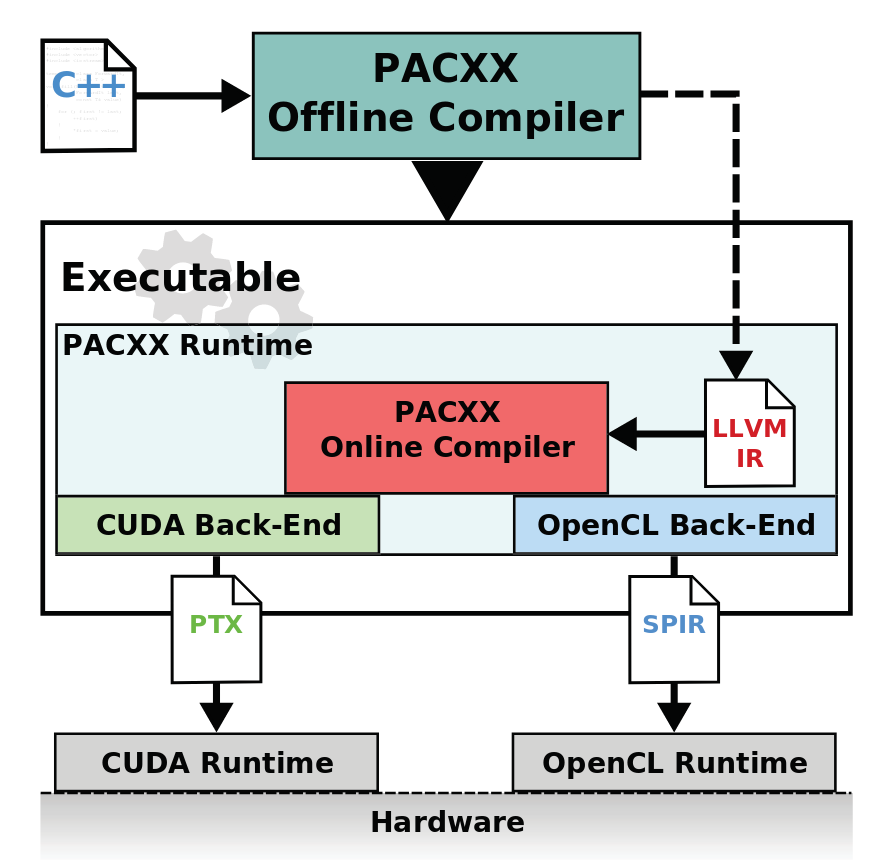
\includegraphics[width=0.8\textwidth]{chapters/relatedWorks/figures/pacxx_compilation_cool.png}
\caption{PACXX Compilation Process\cite{pacxxPaper2}.}
\label{fig:pacxxCompilation}
\end{figure}

\subsection{Key Points}
\textit{PACXX} allows a developer to write device specific code with \textit{C++14} lambdas with few restrictions, and must still take threads and blocks into account. 

\textit{PACXX} uses \textit{LLVM} to generate \textit{PTX} and \textit{SPIR} code at run-time. This is interesting as it provides more opportunities and freedom for abstractions than a static header library would. \textit{PACXX} is also multi-staged such that run-time compiled kernels can vary depending on state.


\chapter{Design Principles}
\label{cha:designPrinciples}
To be able to make informed choices when we design and implement \textit{YAGAL}, we need a vocabulary to explain qualities, and we need to understand what is considered a good API.

\chapter{Framework Design}
The design of the framework, including API and architecture, is described in this chapter. The thought process behind decisions are included here to provide reasoning for the choices when multiple options are present.

%We make decisions, not war!
%
%Language choice:
%C/C++ is the language in focus since it interfaces directly to OpenCL/CUDA, which in turn makes it easier for the developer to substitute the library use with OpenCL/CUDA later in their development process. 
%
%Library design:
%The library is developed following the principles of Cognitive Dimension of Notations. 
%\todo[inline]{Måske også Standard C++ Library Design Guidelines fra isocpp.org, eller revurderede kriterier fra sidste semester}
%
%Implementation plan:
%Using LLVM’s abillity to provide Code Generation from llvm IR to PTX, and using the library to emmit llvm IR.
\section{Design Approach}
We consider the \textit{YAGAL} framework as a combination of two entities; API and architecture.

The API is the front end of the framework, which is what a developer is going to see when using the framework. Designing the API is the task of defining the programming model of the framework, including what functions and types are made available to developers. The API design dictates the usage and learning experience for developers, and many principles exist to guide the development of this part. \todo{refer to previous chapter where we hopefully will define some of these principles.}

The architecture is the structure of the framework, its run-time environment, its compilation process, and platform support. Architectural design decisions will define which use cases are possible to facilitate, and have an impact on how a developer is going to incorporate the framework into her work flow.

\subsection{Design Order}
As both the API and the architecture decisions have an influence on what is possible when designing the other, the order of which these get designed is important. Different approaches is discussed here.

\subsubsection{API First}
When the API is designed before the architecture, we expect the following pros and cons, in no specific order:

Pros:
\begin{itemize}
\item The API will be convenient for the user to use.
\item The API will be simple.
\item The API will not let implementation details propagate.
\item The architecture will have very specific tasks to comply.
\end{itemize}

Cons:
\begin{itemize}
\item The architecture can be limited due to some API decisions being unfeasible on some platforms.
\item The usage might be too far away from the implementation, making some computations more expensive than needed.
\item The requirements to the architecture might be impossible or self conflicting.
\item The API design might require features that make the compilation process convoluted for the developer.
\end{itemize}

In general, this approach is more likely to make our framework ergonomic to use, but it might be at at the cost of architectural simplicity. 

\subsubsection{Architecture First}
When the architecture is designed before the API, we expect the following pros and cons:

Pros:
\begin{itemize}
\item The framework structure will be simpler to explain.
\item Performance optimizations will be more convenient to implement.
\item Allow a convenient tool chain, with a well defined compilation process.
\end{itemize}

Cons:
\begin{itemize}
\item The API design might have implementation details revealed.
\item The API design might be constrained, due to limitations in the architecture.
\end{itemize}

In general, this approach is more likely to make our framework consistent, but it might come at a cost in the form of limitations in the API. 

%\subsubsection{Intertwined}
%When we design them at the same time, and allow design decisions of one to influence the other, we expect the following pros and cons:
%
%Pros:
%\begin{itemize}
%\item A coherent API design and architecture design.
%\end{itemize}
%
%Cons:
%\begin{itemize}
%\item Implementation details might be included in the API design.
%\end{itemize}

\subsubsection{Decision}
As the goal of this project is to make a framework that makes it fast and simple to try GPGPU accelerated code, we choose to design the API first, as it will put the ergonomics of the framework first. As making the underlying architecture work is an implementation problem for us, it is not a concern for a developer.
\section{API Design}
In this section we discuss the design of the API, and the reasoning that behind to these decisions.

\subsection{Goals}
As it is stated in the motivation in Section \ref{cha:motivation}, we want to prioritize high abstraction over absolute performance. W want to avoid exposing kernel logic and put a layer of abstraction upon the general GPU model by handling kernel function setup and setup of blocks and threads for the developer.

In Section \ref{cha:languageSelection} it is stated that we want the API to be replaceable by more specific implementations written in \textit{CUDA}, as such it is preferred that the API allows an easier transition, by allowing interfacing with \textit{CUDA}.

There are multiple ways of achieving a higher level of abstraction and multiple ways of interfacing with \textit{CUDA}. In the following sections we discuss some of the options and decisions taken in designing \textit{YAGAL}.

\subsection{Data types}
We want to provide a developer with types that makes it convenient to work with the GPU. It is difficult to define what makes types accessible and easy to work with since there are multiple factors in play, such as the context of the programming language, the context of application, and what an individual developer sees as convenient. In this section and subsections, we explore some of these factors in the form of memory model, the actual data types, how types are accessed, and compatibility degree for CUDA, in order to determine how the types of \textit{YAGAL} should be designed.

\subsubsection{Memory Model} \label{memoryModelDesign}
% where is the data
Two general directions of handling the underlying memory of \textit{YAGAL}s data types. One is that the data types represent a unified memory layout, where the actual location of the data is handled by \textit{YAGAL}, involving any data transfers required to perform computations. The other is to provide methods for a developer to control the location of the data, giving her more work, but more explicit control. 

% Handle memory implicitly - Bolt and PACXX
In the case of \textit{YAGAL} being able to handle memory transfers between host and device implicitly, data should be available and behave as regular \textit{STL} data types when used on host, and be available for use on device. \textit{Bolt} and \textit{PACXX} handle memory this way, as seen in Chapter \ref{cha:relatedWorks}. An advantage of this approach is that a developer does not need to be concerned about memory when working with \textit{YAGAL}. A downside is that the developer loses control of when transfers are happening, which can come at a high performance cost. It may also create difficulties for a developer when she want to replace \textit{YAGAL} with \textit{CUDA}.

% Provide methods for memory handling - Thrust, AMP, and SkelCL
Memory in \textit{C++} is handled explicitly, and an experienced \textit{C++} developer is used to know and be in control of how and where data is stored. As \textit{YAGAL} is a \textit{C++} library, it makes sense to let developers handle memory themselves. Based on this we decided that \textit{YAGAL} will facilitate ways to manually manage where data is allocated and be able to control transfers between host and device. In Chapter \ref{cha:relatedWorks} we saw that \textit{Thrust}, \textit{C++ AMP}, and \textit{SkelCL} handles memory this way.

% The decision
We decided that \textit{YAGAL} will provide developers with the means to manage allocation and transfers of data between host and device themselves, instead of handling it implicitly.

\subsubsection{Supported Types}
% Introduction to considered types
There are many types that \textit{YAGAL} potentially can provide. To stay within the time frame of this project, we decide to keep the current amount of provided types to a minimum, and extend \textit{YAGAL} with additional types depending on the deadline. The types we have considered are \texttt{arrays}, \texttt{vectors}, and \texttt{maps}.

% We would like vectors, but arrays if it fails
\texttt{vectors} are contiguous memory that can be used as arrays with the possibility of being dynamically resized, in contrast to \texttt{arrays} which are contiguous memory with a static size. The frameworks in Chapter \ref{cha:relatedWorks} all provide \texttt{vectors} with the exception of \textit{C++ AMP} that uses \texttt{arrays} and \texttt{array\_views}. Based on this, we want \textit{YAGAL} to support \texttt{vectors}, but it is unclear to what degree of complications the implementation of \texttt{vectors} would introduce, due to their dynamic functionality. \texttt{arrays} on the other hand, appear to be more simple to implement due to them being statically sized. We will therefore focus on implementing \texttt{vectors} and have \texttt{arrays} as fallback solution, as the possibility of being able to dynamically resize a data collection is a quality that makes it easier for developers to use.

% Multi dim support
In regard to multidimensional support for \texttt{vectors} and/or \texttt{arrays}, it is convenient to have as it makes some tasks easier to implement, but it is of low priority as it is a more specialized feature, that is not needed by all developers, in contrast to single dimension arrays or vectors. We would useful for \textit{YAGAL} to support it, but it will not be prioritized.

% No support for maps
The \texttt{map} data container is an interesting option, since the GPU could be utilized to perform lookups. This however does not contribute to the overall goal of \textit{YAGAL}, as we have not observed this feature in any of the tools covered in chapter \ref{cha:relatedWorks} and the introduction of this feature does not contribute to \textit{YAGAL} being replaceable. \texttt{map} will therefore not be supported.

\subsubsection{Accessing Data}
When a data container is in use, there are multiple possible methods of accessing the data that can be expected. 

When a single element is required, either for read or write, we consider two options:
\begin{itemize}
\item Using \texttt{container.get(index)} and \texttt{container.set(index, value)} to read and modify.
\item Using \texttt{container[index]} to read and modify.
\end{itemize}
We chose to implement get and set functions, as the square bracket accessing can be developed on top of these at a later point if needed.

It is more problematic when more than a single element is needed. There are multiple options we consider:
\begin{itemize}
\item Providing iterators to provide iteration over data, as is tradition in \textit{C++}.
\item Providing a pointer to the first element and a number of elements to let a developer control access, as is tradition in \textit{C}.
\item Providing the number of elements to let the developer use single element accessing methods.
\item Providing casting rules to let a developer cast a collection to another type that provides the needed accessing methods at the cost of a data transfer to host.
\end{itemize}
We chose to provide a developer with the device pointer to the data, and the number of elements contained, giving the developer information enough to use the single element accessors. This also allow direct access to the memory for other frameworks if multiple frameworks are used together.

Providing iterators is problematic as it motivates the developer to make many small copies back and forth between device and host. Instead we chose to provide a method to create a \textit{STL} vector with a copy of the device data, which will provide iterators for the copy. The copy can then be copied back to the device, and as such only need two transfers, which compared to two transfers per element is more convenient.

\subsection{Functions}
To let a developer use \textit{YAGAL} we need some functions to provide the needed functionality. We chose to experiment with a different function structure compared to the related works in chapter \ref{cha:relatedWorks}. Where the related works generally define some kind of kernel function, and then applies it to a collection, we want to build the kernel on the collection in an attempt to make the process more readable.

\subsubsection{Calling execute on a collection}
% Principle
A way to achieve building a kernel upon the collection could be by doing it lazily. A developer could build up kernel functionality by appending functions upon the collection. When the developer have applied her functions, then the actual kernel function would be generated and executed based on the stored functions, when she calls execute on the collection.

% Pros
An advantage of this approach is that it could prevent unnecessary data transfers between host and device since it might be possible to bundle necessary logic within a single kernel function. 

% Cons 
A disadvantage of this approach is that it could be a cause for confusion for the developer. When the developer applies \texttt{add(5)} to a collection, a developer might expect the addition to have already taken place.

\subsubsection{Function Chaining}
We want to make a single kernel able to execute multiple actions, such as adding and multiplying a value in sequence. To enable this we want each function call to return a reference to the collection object so that multiple actions can be queued before the final execute call.

This will allow a program, that adds 5 to all elements of a collection before multiplying them with 2, in \textit{YAGAL} to be written as \texttt{collection.add(5).multiply(2).exec()}, which we find to be very intuitive to read in comparison to the define kernel and apply kernel form of the other frameworks.

Allowing chaining of functions also allow the framework to make decisions on how to split kernels, so that the example above would result in executing a single kernel doing both actions, rather than executing an add kernel and a multiply kernel in sequence.

\subsubsection{?}
\todo{Hvilke low order functions vil vi have}

\subsubsection{?}
\todo{Hvilke high order functions vil vi have}

\section{Architecture Design}
In this section we discuss the decisions made regarding the architecture of \textit{YAGAL}, including compilation method, run time, and compatibility.

\subsection{Using LLVM and CUDA Driver API}
In chapter \ref{cha:relatedWorks} we see that there are frameworks which use \textit{LLVM} to build a compiler that output either \textit{PTX} or \textit{SPIR} code. We also see that there are frameworks that without introducing a compiler translates to \textit{OpenCL} code. We have not found any that without a compiler translates to \textit{CUDA} or \textit{PTX}, we want to attempt this.

As \textit{LLVM Intermediate Representation} is a higher level language than \textit{PTX}, we still want to make use of \textit{LLVM}. The idiomatic use of \textit{LLVM} is to build a compiler with the passes provided by the \textit{LLVM}, and additional passes defined by the compiler developer, but as we want to avoid building a compiler that a developer is forced to use to use our framework, we can not do this. Instead we want to use the \textit{LLVM} framework by including it in our library in such a way, that the user of \textit{YAGAL} compiles the necessary components of \textit{LLVM} into her executable. This allow us to generate \textit{LLVM Intermediate Representation} and use \textit{LLVM}s back-ends to target \textit{PTX} inside the \textit{YAGAL} library.

When we can generate \textit{PTX} we can focus on executing it, which is done using the \textit{CUDA Driver API}. The \textit{CUDA Driver API} differ from the \textit{CUDA Runtime API} by being slightly more verbose, but allowing \textit{PTX} to be invoked, and not requiring the \textit{NVIDIA} compiler. Using the \textit{LLVM} library in conjunction with the \textit{CUDA Driver API} allow us to handle code generation and execution without requiring a specific compiler.

Using the \textit{LLVM} library and the \textit{CUDA Driver API} does impose dependencies that the user of \textit{YAGAL} is required to have available. So while the compiler choice is still up to the developer, the need to install these two libraries are still present as a prerequisite to using \textit{YAGAL}.

Figure \textit{fig:architectureOverview} illustrate an overview of \textit{YAGAL}. We show that the source is clean \textit{C++} with nothing but \textit{YAGAL} library inclusion. This source, when compiled, result in a executable that contains the logic of the program, together with the \textit{YAGAL} logic to both generate \textit{LLVM Intermediate Representation} and manage memory, together with the \textit{LLVM Translator} which translates the \textit{LLVM Intermediate Representation} to \textit{PTX}. The run-time requirement of a \textit{CUDA Driver} is present as it is the part that facilitates memory management and code execution on the GPU.

\begin{figure}[H]
\center
\includegraphics[width=0.8\textwidth]{chapters/frameworkDesign/figs/architecture.png}
\caption{Architectural overview of YAGAL.}
\label{fig:architectureOverview}
\end{figure}


\subsection{CUDA Compatibility}
In cases where programs are unable to be expressed in \textit{YAGAL}, we want to provide a fall back solution. We intend to do this though letting the developer execute arbitrary \textit{PTX} code, through the \textit{CUDA Driver API}. To allow this we want our abstractions to provide access to the relevant device pointers to the GPU.

This solution still require the developer to have \textit{PTX} code that solves the problem. Normally this would mean writing \textit{CUDA} code, and compile that to \textit{PTX}, which is a long work around. As such it is not ideal, but we decide that it is better to provide a problematic work around, rather than none.

\chapter{Framework Implementation}

The framework implementation were performed in incremental steps, as described in chapter \ref{cha:developmentProcess}. This chapter contain implementation details of the steps in order of completion.

\chapter{Framework Comparison}
\todo{Comming soon}

Find ud af hvad der skal sammenlignes.

Points to compare:
\begin{description}
\item[Performance]
\item[Lines of code]
\item[Size of executable]
\item[Programability]
\end{description}


\chapter{Demo application}
\todo{Comming soon}

\chapter{Evaluation}
Here we do stuff like, saying it works, and it goes THAT fast!
\section{Test}
We actually did some tests, and respected the nice feedback from our previous examn.

\section{Performance}
Oh yeah? this one is actually THIS fast!

\chapter{Reflection}
Actually, starting with weird dummy texts in files, was a pretty good idea!

\chapter{Conclusion}
\todo{genetabler problem og hvad vi vil}
GPGPU development is not an easy task, and present a steep learning curve for a developer getting into it. There are multiple frameworks that attempt to solve this, and they do this by providing various higher level constructs. These frameworks have different dependencies and requirements that the developer must fulfill, including compiler and run-time requirements. 

In this project we perform an experimental design and implementation of \textit{YAGAL}, with the aim of being compiler-independent with a comprehensible programming model with design decisions not covered by related work.

The project started based on the problem statement:

\todo{paste problemformulering}
\textit{Can a GPGPU framework to abstract the underlying programming model be created, as a library that does not limit the developers choice of compiler, and how does it compare to other frameworks that do?}

\todo{hvilke opageaver vi skulle løse for den}
Throughout the project we have worked with the following tasks, which have been derived from the problem statement:

\todo{gå gennem hvert løst punkt}
\begin{description}
\item[Create an overview of related works]\hfill \\
We have identified a set of frameworks that provide abstractions for GPGPU development, and analyzed their qualities.
\item[Research framework design principles]\hfill \\
We have identified a set of design principles that we have followed during development.
\item[Design the framework]\hfill \\
We have designed \textit{YAGAL} with a novelty not found in the related works. \textit{YAGAL} is the result of our choice of compilation method and used technologies, prioritizing experimentation over features.
\item[Implement the framework]\hfill \\
We have implemented a major subset of the design, and provided a discussion about methods of proceeding regarding the discovered problems. 
\item[Implement demo application]\hfill \\
We have implemented an algorithm to show the features of \textit{YAGAL}, and to provide material for evaluating and comparing \textit{YAGAL} to the related works.
\item[Evaluate the design and implementation of the framework compared to related works]\hfill \\
We have evaluated \textit{YAGAL} in regards to measured performance and usability, using the cognitive dimensions of notations, and compared it to the related works.
\end{description}

\todo{praleblock}
%yagal drømmen, compilerfriiiiiii, fucking unikum
We have designed \textit{YAGAL} to be an compiler-independent framework, with a run-time based on the \textit{CUDA Driver API}. None of the related works that utilize \textit{CUDA} are compiler independent, which is what inspired this combination.

%yagal abstractionen
We have provided abstractions for both the memory management in the form of a vector construction, and the construction of kernels in the form of actions. A developer does not have to perform manual allocation and copies on the device, our vector construction handles those tasks for her. A developer also do not have to learn the kernel abstraction of a lower level framework such as \textit{CUDA} or \textit{OpenCL}, as she can apply transformations on our vectors using our actions as building blocks to express the kernel logic.

%llvm smadder brug
We have utilized the \textit{LLVM} library to provide an intermediate representation, for our generated kernels. For our run-time \textit{PTX} code generation, we have made a single purpose re-implementation of \textit{LLVM llc}, which get packaged in the final executable.

%hvilke problemer opdagede vi? og vi præsenterer løsningsforslag
We have discovered that targeting a language that is not \textit{OpenCL} without introducing a compiler results in anonymous functions being problematic to implement. We have proposed a set of possible solution strategies for this problem, including the expected difficulty and implications.

\todo{konkluder betragtninger}
Finally we conclude that it is indeed possible to create a compiler-independent framework that utilize the \textit{CUDA Driver API}, but when high level abstractions are needed, those require significantly more work to implement compared to other designs.


\chapter{Future Work}
This chapter contain the topics that need to be addressed in the future, if the development on \textit{YAGAL} were to continue.

\todo{Undersøg om der virkeligt er behov for en sådan løsning, vi tog udgangspunkt i at der ikke var noget, ikke at det manglede}

\todo{Implementer lambdaer. Flere muligheder som nævnt i cha?? men meget tidskrævende, hvis ikke det er den billige løsning (nvrtc)}.

\todo{Når funktionaliteten er til det, sørg for at vi følger med performance wise... thrust er gud.}

\printbibliography

\part{Appendix}
\appendix

\end{document}
